% (c) GreenSocs Ltd
% author: Christian Schroeder <schroeder@eis.cs.tu-bs.de>

\section{Requirements for the GreenConfig Configuration Framework}
\label{requirements}

\subsection{Definitions}Before we start, we need some definitions: 


\subsubsection{Tool}
We can consider two types of tools: 

\begin{itemize}
	\item {\em Internal} tools, i.e. a configuration/debug library linked to the model  
	\item {\em External} tools may assist in verification of the model by providing increased visibility and control during simulation, and assisting the user in configuring the model in various ways before and during simulation. 
\end{itemize}


\subsubsection{Configurable Parameter}
By the term configurable parameter we denote sc\_module members that can be accessed (get/set value) by means of a config API.  


\subsubsection{Config API}A config API is an interface to a configuration framework with the goal, that  

\begin{itemize}
	\item the user can create and access (get/set) parameters 
	\begin{itemize}
		\item during construction/elaboration 
		\item at simulation runtime 
	\end{itemize}
\end{itemize}

Additional features may include 

\begin{itemize}
	\item tracking of parameter value changes (e.g., using event notification or callbacks) 
	\item initialize parameters from a configuration file 
	\item search for parameters in the model 
	\item get a list of all parameters in the model 
	\item dump parameters to a trace or config file 
	\item add constraints / assertions to parameters 
	\item synchronize parameters between SystemC model and external tool (push / pull) 
	\item ... 
\end{itemize}

Examples for different config APIs are: 

\begin{itemize}
	\item CoWare SCML 
	\item ARM CASI \item Intel DRF \item GreenSocs Simple Configuration Framework 
\end{itemize}

\begin{figure}[H]%[htbp]
	\centerline{
		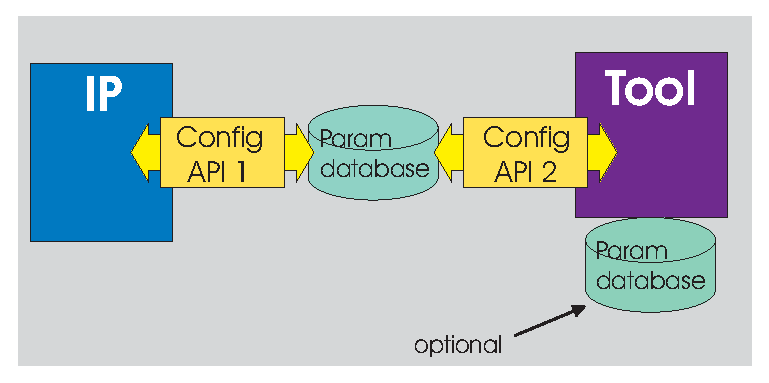
\includegraphics[width=10cm]{requirements_API_overview.eps}} 
	\caption{Overview configuration in general.}
	\label{fig:overviewAPIrequ}
\end{figure}



\subsection{Basic idea: the GreenConfig Core}
The \GreenConfig Core implements all functionality required to manage configurable parameters in SystemC models (implementation details follow below). It provides a generic GC-API which is used to built heterogeneous User APIs on top of it.  

Hence it has to be well designed to support virtually all functions other APIs might ask for. {\bf User API adaptors} translate between the \GreenConfig framework and the vendor's interfaces / APIs. 

\begin{figure}[H]%[htbp]
	\centerline{
		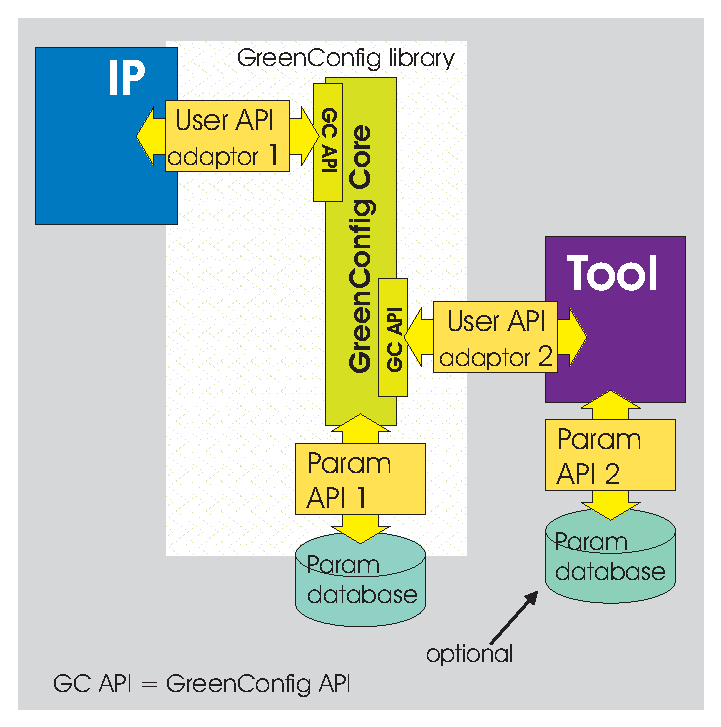
\includegraphics[width=10cm]{requirements_API_overview_GreenConfig.eps}} 
	\caption{Overview configuration with GreenConfig library.}
	\label{fig:overviewGreenConfrequ}
\end{figure}



\subsection{Main requirements}
\begin{itemize}
	\item Support {\em most} config APIs (as much as reasonable regarding effort) 
	\item Ease of use (i.e. usage requires minimal to no additional implementation effort) 
	\item Extensibility (e.g., support more data types, add new config file formats, add additional functionality) 
\end{itemize}



\subsection{Requirements classification}
We consider three classes of requirements: 

\begin{enumerate}
	\item Requirements for \GreenConfig to support known configuration APIs 
	\item Functionalities we from our point of view would like to see in \GreenConfig  
	\item Requirements for future directions 
\end{enumerate}



\subsubsection[(1.) Requirements to support other parameter configuration APIs]{(1.) Requirements for \GreenConfig to support other parameter configuration APIs}
\label{lab:requ1}
Table \ref{tbl:capabilitiesa} is based on the spreadsheet searching\_configurations\_in\_SystemC.xls 

These requirements (\ref{lab:requ1}) are made from the view of supporting the tool and user APIs of all other vendors. 

\begin{itemize}
	\item Provide an interface for the user and the tool (eventually uniform interface). This '\GreenConfig API' named interface is \GreenConfig internal and is used by the specialized 'User API adaptor' for a special vendor. The GC API has to support all thinkable functionality of any user and tool API of any vendor. 
	
	\item Interface to user API (\GreenConfig User API adaptor 1, see figure \ref{fig:overviewAPIrequ}) must allow: 
	
	\begin{itemize}
		\item Registering a parameter (The user can add a parameter to the configuration framework.) 
		\item Set default value (Set value of a parameter during elaboration) 
		\item Get value (Get the initial value of a parameter; set by default value or by tool) 
		\item Change value during runtime (The user may change value of a parameter even during simulation runtime.) 
		\item Notify changes to user (Register observer for a parameter either a parameter of the own module or a parameter of another module.) 
	\end{itemize}
	Interface to tool API (\GreenConfig User API adaptor 2, see figure \ref{fig:overviewAPIrequ}) must allow: 
	
	\begin{itemize}
		\item Configuration during elaboration / runtime (Set value of a parameter during elaboration and runtime) 
		\item Notify changes to tool (Register observer for a parameter which can be changed by the user during runtime) 
		\item Get value during elaboration / runtime (Get the value of a parameter during elaboration and runtime) 
		\item This interface may be used by a GUI tool 
	\end{itemize}

	\item The User API adaptors must be specialized for each vendor, using the \GreenConfig API and providing the vendor's APIs. 
\end{itemize}

\begin{landscape}
\begin{table}[H]
	\begin{tabularx}{23cm}{|X|X|X|X|X|X|}
		\cline{1-1}\cline{2-2}\cline{3-3}\cline{4-4}\cline{5-5}\cline{6-6}
		               & \multicolumn{5}{|l|}{ supported by    }\\ 
		\cline{1-1}\cline{2-2}\cline{3-3}\cline{4-4}\cline{5-5}\cline{6-6}
		               & {\bf Co\lstinline||Ware}   & {\bf ARM}   & {\bf TI} \newline no parameters   & {\bf Intel}   & {\bf GreenS. Simple \newline Config. \newline  Framew.}  \\ 
	
		\cline{1-1}\cline{2-2}\cline{3-3}\cline{4-4}\cline{5-5}\cline{6-6}
		Data types     & int, unsigned int, \newline double, bool, std::string    & std::string    & unknown, however \href{http://www.greensocs.com/SystemC/SystemCEvents/DATE2007Slides?action=AttachFile\&do=get\&target=systemPython-date-presentation-07.ppt}{presentation}  \newline implies that strings and  \newline number formats are supported   & "Instrumented Datatype" \newline user implemented \newline implement interfaces   & PODs, STL, SystemC  \\ 
		\cline{1-1}\cline{2-2}\cline{3-3}\cline{4-4}\cline{5-5}\cline{6-6}
		User defined types   & -   & yes (user implemented)   &     & yes (instrumented data type)   & yes (template specialized)  \\ 
		\cline{1-1}\cline{2-2}\cline{3-3}\cline{4-4}\cline{5-5}\cline{6-6}
		Permanent storage    & XML   & -   & -   & file   & file  \\ 
		\cline{1-1}\cline{2-2}\cline{3-3}\cline{4-4}\cline{5-5}\cline{6-6}
		Registering a parameter   & yes (global registry)   &  yes    &  -    &  drf module finds  \newline parameters itself   & yes (\lstinline|addParam| or macro \lstinline|GB_PARAM|  \\ 
		\cline{1-1}\cline{2-2}\cline{3-3}\cline{4-4}\cline{5-5}\cline{6-6}
		Set default value        & yes (constructor)   & user may implement   & user may implement   & yes   & yes (constructor)  \\ 
		\cline{1-1}\cline{2-2}\cline{3-3}\cline{4-4}\cline{5-5}\cline{6-6}
		Get value   & yes (e.g. \lstinline|getIntProperty(key)|   & yes (\lstinline|getParameter| \newline \lstinline|(string key)|)   & yes (pushed by method call)   & yes (Interface I\_dr\_dump)   & yes (\lstinline|get|)  \\ 
		\cline{1-1}\cline{2-2}\cline{3-3}\cline{4-4}\cline{5-5}\cline{6-6}
		Config. during runtime \newline Done by other module or tool   & -   & -   & yes (task\_start)   & -   & yes (\lstinline|set|)  \\ 
		\cline{1-1}\cline{2-2}\cline{3-3}\cline{4-4}\cline{5-5}\cline{6-6}
		Change value during runtime \newline Done by module itself   & yes   & yes (user implemented)   & yes (user implemented)   & yes (user implemented)   & yes (\lstinline|set| or direct)  \\ 
		\cline{1-1}\cline{2-2}\cline{3-3}\cline{4-4}\cline{5-5}\cline{6-6}
	\end{tabularx}
	\caption{(a) This spreadsheet shows the capabilities of the reviewed configuration systems.}
	\label{tbl:capabilitiesa}
\end{table}

\begin{table}[H]
	\begin{tabularx}{23cm}{|X|X|X|X|X|X|}
		\cline{1-1}\cline{2-2}\cline{3-3}\cline{4-4}\cline{5-5}\cline{6-6}
		               & \multicolumn{5}{|l|}{ supported by    }\\ 
		\cline{1-1}\cline{2-2}\cline{3-3}\cline{4-4}\cline{5-5}\cline{6-6}
		               & {\bf Co\lstinline||Ware}   & {\bf ARM}   & {\bf TI} \newline no parameters   & {\bf Intel}   & {\bf GreenS. Simple \newline Config. \newline  Framew.}  \\ 
	
		\cline{1-1}\cline{2-2}\cline{3-3}\cline{4-4}\cline{5-5}\cline{6-6}
		Notify changes to user   & -   & -   & yes (task call)   & yes (event as member of instr. datatype)   & -  \\ 
		\cline{1-1}\cline{2-2}\cline{3-3}\cline{4-4}\cline{5-5}\cline{6-6}
		Configuration during elaboration   & yes (instantiation, with global registry)   & yes (in user module \lstinline|setParameter(string| \newline \lstinline|key, string value)|)   & no (but task\_start)   & yes (Interface I\_dr\_config)   & yes (constructor or \lstinline|set|)  \\ 
		\cline{1-1}\cline{2-2}\cline{3-3}\cline{4-4}\cline{5-5}\cline{6-6}
		 / runtime   & -   & -   & method calls   & -   & yes (\lstinline|set|)  \\ 
		\cline{1-1}\cline{2-2}\cline{3-3}\cline{4-4}\cline{5-5}\cline{6-6}
		Notify changes to tool   & -   & -   & task-finished event   & -   & -  \\ 
		\cline{1-1}\cline{2-2}\cline{3-3}\cline{4-4}\cline{5-5}\cline{6-6}
		Get value during elaboration    & -   & -   & -   & yes (dump)   & -  \\ 
		\cline{1-1}\cline{2-2}\cline{3-3}\cline{4-4}\cline{5-5}\cline{6-6}
		 / runtime   & -   & -   & -   & yes (dump)   & -  \\ 
		\hline
	\end{tabularx}
	\caption{(b) This spreadsheet shows the capabilities of the reviewed configuration systems.}
	\label{tbl:capabilitiesb}
\end{table}
\end{landscape}




\subsubsection{(2.) Requirements for GreenConfig in General from bottom-up}
\label{lab:requ2}
These requirements describe the framework from our view without regarding special other APIs but to achieve a many-sided framework. 

\begin{enumerate}
	\item {\em Usage} 
	\begin{enumerate}
		\item New datatypes can be easily added by the user (to provide as many datatypes as possible) 
		\begin{enumerate}
			\item Methods to set and get the value of the parameter use \lstinline|std::string|: \newline  void set(const std::string \&str) and const std::string get()  \newline  This allows easy adaption of the tools to set a parameter and is universal. 
			\item The data type of a template should be given as template parameter.  \item Usage of a templated parameter (\lstinline|gs_param<datatype>|) should be as easy as the usage of the data type itself by overloading the operators (\&, =). This is the instrumentation of a member variable to use it as a parameter. The usage of the parameter is transparent due to the overloaded operators. (SOW 3.1.3) 
		\end{enumerate}
		\item Support all imaginable parameter types and usages, e.g. 
		\begin{itemize}
			\item Setup parameters: Setup parameter is set during elaboration. The module complies with the value of the parameter to act variedly. 
			\item Change setup parameters: Parameter which changes during runtime to take influence on the behavior of the module. 
			\item Status parameters: Status parameter represent the status of a module. They are set by the module itself. Observers are notified when it changes. 
			\item Output parameters: Parameters to send output (debug values etc.) to the tool outside the simulation. 
			\item ... 
		\end{itemize}
	\end{enumerate}

	\item {\em Configuration} 
	\begin{enumerate}
		\item Configuration during elaboration 
		\item Configuration during runtime 
		\item Use same configuration system (same methods etc.) for initial configuration during elaboration and runtime configuration during simulation 
		\item Provide setting of parameters to other IPs (e.g. tools) 
		\begin{itemize}
			\item Setting of a parameter: \lstinline|setParameter(std::string hierarchical_name, std::string value)| 
		\end{itemize}
		\item Provide getting of parameter values to other IPs (e.g. tools) 
		\begin{itemize}
			\item Getting of a parameter value: \lstinline|std::string getParameter(std::string hierarchical_name)| 
		\end{itemize}
		\item Provide setting of parameters inside user code. There are two different types: 
		\begin{enumerate}
			\item Setting of the parameter in the module which contains the parameter: \newline Inside the parameter holding module the user may choose out of two ways of setting the value.  
			\begin{itemize}
				\item The user can set the value with the setting method (see requirement 1.1.1) using the parameter's string representation. 
				\item The value can be set with the instrumentation of the member variable by simply assigning the value (see requirement 1.1.3). 
			\end{itemize}
			\item Setting of the parameter of module in another module
						 We have two options to realize the access to parameters of another module: First we can access them directly by pointer. This assumes the availability of the pointer which has to be provided by a central unit. It is clearer to provide the setting of a parameter by a function contained in the API of the library. Here the same method can be used which is also used by the tool API to set parameters (see requirement 2.4). 
		\end{enumerate}
		\item A default value can be set during instantiation/construction of the parameter: \lstinline|gs_param(const char *name, T value)|. 
	\end{enumerate}

	\item {\em Core} 
	\begin{enumerate}
		\item Efficient data management (database) for runtime (how parameters are saved during runtime, e.g. map, list,...) 
		\item Efficient data management (database) for permanent storage (e.g. config file, XML file, Access database,...) 
		\item Find local and global identification system for parameters (names): Unique name inside module, full name composed of hierarchical names leading to parameter name (\lstinline|module_name.submodule_name.parameter_name|) 
		\begin{itemize}
			\item Name a parameter during instantiation with \lstinline|my_param = gs_param<datatype>(my_name)|. 
			\item Get the parameter name with \lstinline|const std::string &getName()|. 
		\end{itemize}
	\end{enumerate}

	\item {\em Observation / notification} 
	\begin{enumerate}
		\item Provide a complete parameter list: e.g. \lstinline|multimap<const char * hierarchical_prefix, const char * name> getParameterList()| or \lstinline|list<std::string hierarchical_name> getParameterList()| 
		\item Allow an observer to register for a parameter to be notified with an event when it changes 
		\begin{enumerate}
			\item Allow many observers per parameter 
			\item Additional one event per configurable module \lstinline|config_changed|? 
		\end{enumerate}
		\item Provide to the module itself an event which is notified when any parameter of the module is changed (function callback {\em and} sc\_event) (see requirement 4.2.2). 
		\item Either the parameters have to register themselves at the library or the library finds the parameters or modules due to the implementation of the config interface (e.g. \lstinline|gs_configurable|). 
	\end{enumerate}

	\item {\em Additional requirements resulting on conference call on 21st May 2007} 
	\begin{itemize}
		\item Secure IPs which allow disabling their configuration abilities. 
		\item Some kind of privacy tags to protect parameters being changes from outside the module. 
		\item Recording actions (who is when setting or getting etc.) in the Core 
	\end{itemize}

\end{enumerate}


\subsubsection{(3.) Requirements for the support of other control interfaces}
These requirements are formed by additional control issues. Here not the parameter configuration must be provided but more general control methods. E.g. configuration or starting a task with the call of a configuration method which is provided by a given or user defined interface . 

This part is for future use and has no priority at this moment. 

\subsection{Sorted and prioritized requirements}

\begin{enumerate}
	\item Default value during construction 
	\item Configuration during elaboration 
	\item Configuration during runtime (Callback/event on change) 
	\item Supported data types (set and get with strings, addition of parameter types easy) 
	\item User defined data types 
	\item Notify changes to tool (Callback/event on change) 
	\item Notify changes to user module (Callback/event on change) 
	\item Permanent storage in file 
\end{enumerate}
